\documentclass[12pt]{article}
\usepackage[a4paper, total={5.5in, 9in}]{geometry}
\usepackage{amsmath}
\usepackage{amsfonts}
\usepackage{graphicx}
\usepackage{pgfplots} % Para crear gráficos
\pgfplotsset{compat=1.18} % Para evitar warnings de compatibilidad
\usepackage{enumitem}

\title{College Algebra Worksheet 3.3}
\author{PCL Learning Center}
\date{}

\begin{document}
\maketitle

\begin{center}
    \textit{note: No graphing calculators or electronic devices may be used on this worksheet.}    
\end{center}

\section*{Problem Set 1\\Difficulty level: Normal}
\subsection*{Problem 1}
Find the difference quotient \(\dfrac{f(x+h)-f(x)}{h}\) for the function given below.
\[f(x)=-x^2+x+2\]

\subsection*{Problem 2}
Given the table of values, find the average rate of change of the function \(f(x)\) on the interval \([4,12]\).

    \begin{center}
    \begin{tabular}{|*{12}{c|}}
    \hline
    % First row (12 columns)
    \(x\) & 3 & 4 & 5 & 6 & 7 & 8 & 9 & 10 & 11 & 12\\
    \hline
    % Second row (12 columns)
    \(f(x)\) & 67 & 81 & 87 & 124 & 141 & 144 & 175 & 194 & 220 & 223\\
    \hline
    \end{tabular}
    \end{center}

\subsection*{Problem 3}
Find the average rate of change of the given function on the interval \([0,2]\).
\[f(x)=-3x^3-x^2+3x\]

\subsection*{Problem 4}
Can the average rate of change of a function be constant? If yes, give two examples.
\newpage
\subsection*{Problem 5}
Find the local maximum of the function \(f(x)\).

\begin{figure}[!ht]
    \centering
    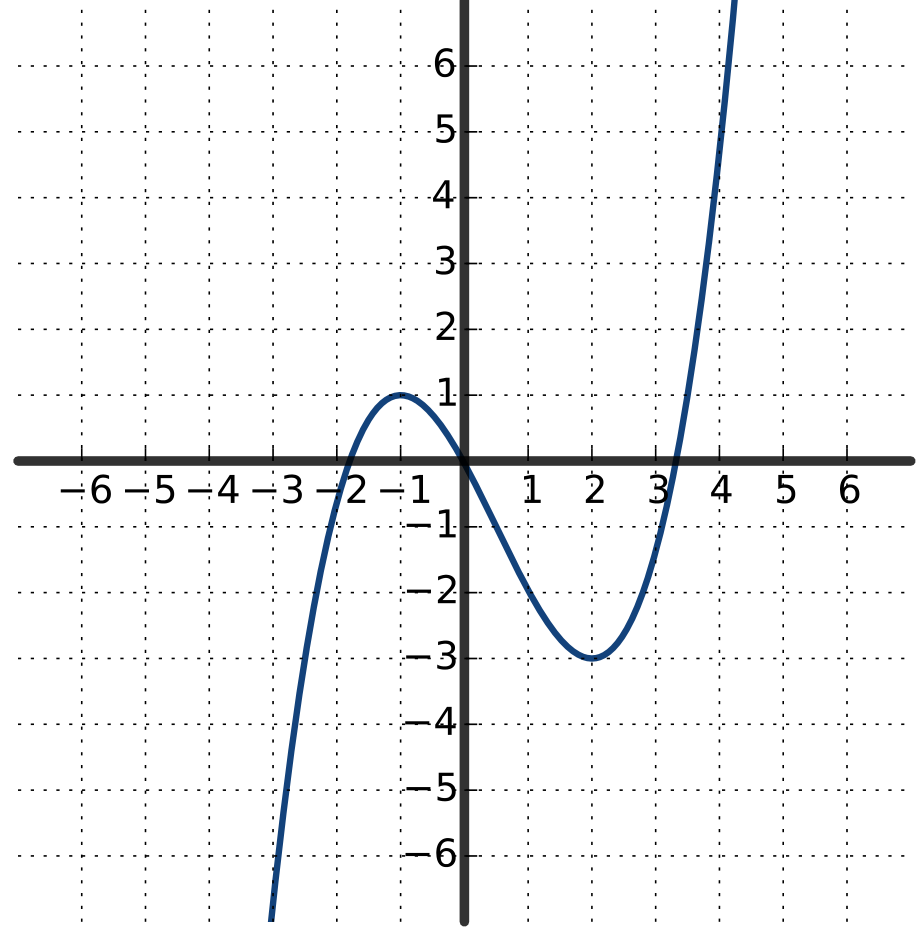
\includegraphics[width=0.5\linewidth]{3.png}
\end{figure}

\subsection*{Problem 6}
Identify the local maximum and local minimum of the function.
\begin{figure}[!ht]
    \centering
    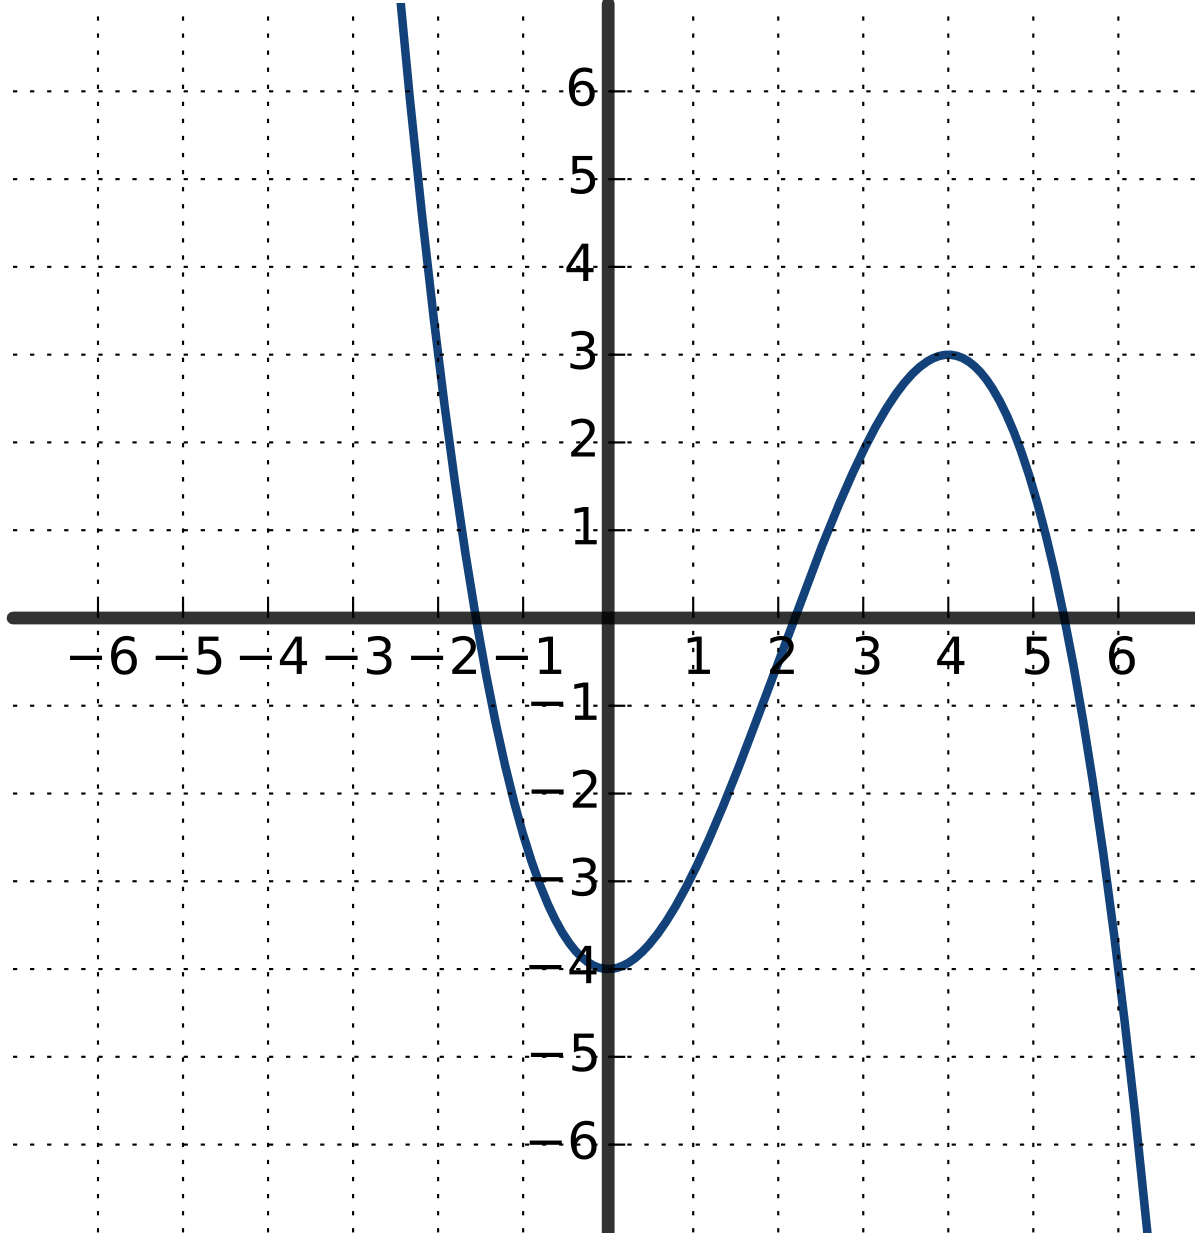
\includegraphics[width=0.5\linewidth]{4.png}
\end{figure}

\subsection*{Problem 7}
Find the absolute maximum value of the function.
\begin{figure}[!ht]
    \centering
    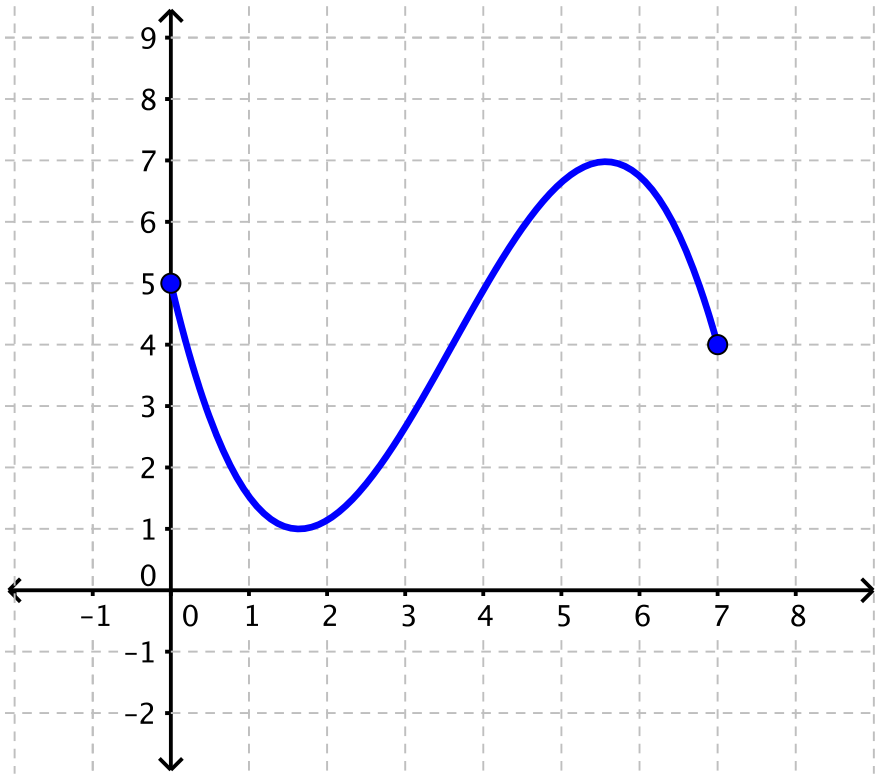
\includegraphics[width=0.5\linewidth]{5.png}
\end{figure}

\newpage
\subsection*{Problem 8}
Determine the intervals where the function is decreasing.
\begin{figure}[!ht]
    \centering
    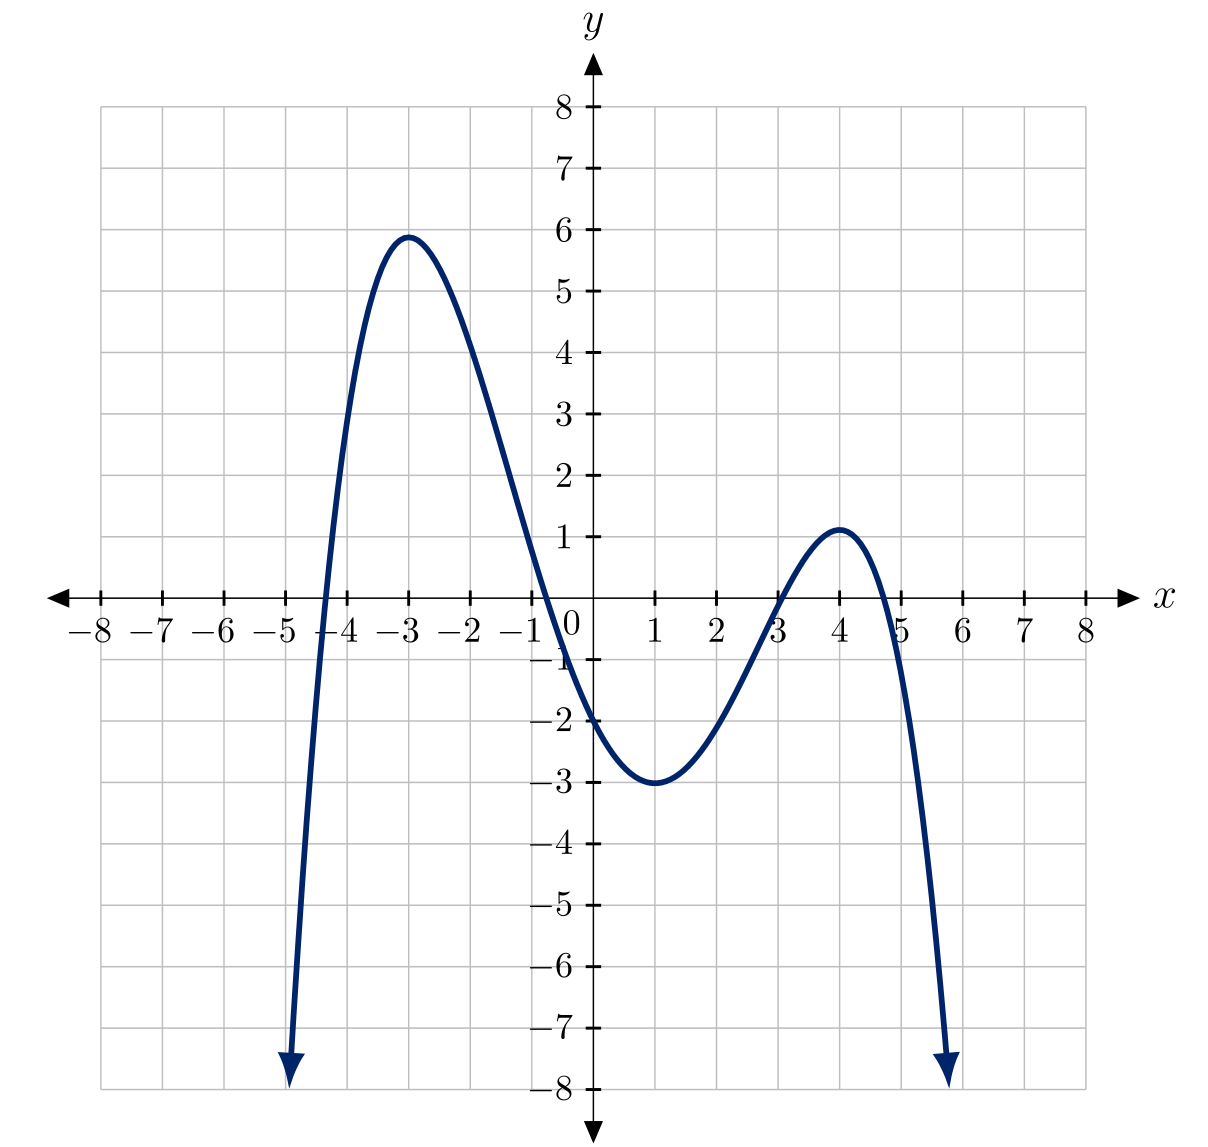
\includegraphics[width=0.5\linewidth]{6.png}
\end{figure}

\section*{Problem Set 2\\Difficulty level: Hard}
\subsection*{Problem 1}
Find the average rate of change of each function on the following intervals.

    \begin{enumerate}
        \item[(a)] \(3x^3\) on \([1,1+x]\)
        \item[(b)] \(4t^3\) on \([2,2+t]\)
        
    \end{enumerate}

\section*{Solutions for the Set 1}
\subsection*{Problem 1}
\(-2x-h+1\)
\subsection*{Problem 2}
19
\subsection*{Problem 3}
-11
\subsection*{Problem 4}
Yes. Consider \(f(x)=x\) and \(g(x)=x+1\).
\subsection*{Problem 5}
local maximum: \((-1,1)\)
\subsection*{Problem 6}
local maximum: \((4,3)\), local minimum: \((0,-4)\)
\subsection*{Problem 7}
absolute maximum: 7
\subsection*{Problem 8}
\((-3,1)\cup (4,\infty)\)

\section*{Solutions for the Set 2}
\subsection*{Problem 1}
\begin{enumerate}
    \item[(a)] \(3x^2+9x+9\)
    \item[(b)] \(4t^2+24t+48\)
\end{enumerate}

\end{document}
